\documentclass[varwidth=true, border=2pt]{standalone}

\usepackage{pgfplots}
\usepackage{tikz}
\usetikzlibrary{patterns}

    \tikzset{
        hatch distance/.store in=\hatchdistance,
        hatch distance=10pt,
        hatch thickness/.store in=\hatchthickness,
        hatch thickness=2pt
    }

    \makeatletter
    \pgfdeclarepatternformonly[\hatchdistance,\hatchthickness]{flexible hatch}
    {\pgfqpoint{0pt}{0pt}}
    {\pgfqpoint{\hatchdistance}{\hatchdistance}}
    {\pgfpoint{\hatchdistance-1pt}{\hatchdistance-1pt}}%
    {
        \pgfsetcolor{\tikz@pattern@color}
        \pgfsetlinewidth{\hatchthickness}
        \pgfpathmoveto{\pgfqpoint{0pt}{0pt}}
        \pgfpathlineto{\pgfqpoint{\hatchdistance}{\hatchdistance}}
        \pgfusepath{stroke}
    }

\begin{document}
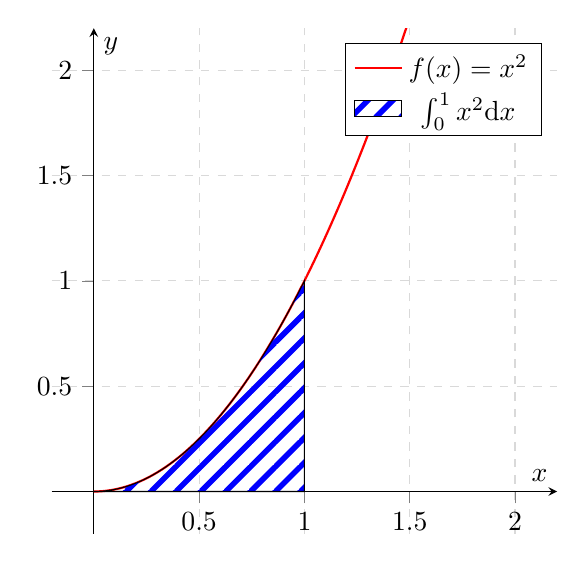
\begin{tikzpicture}
    \begin{axis}[
        legend pos=north east,
        axis x line=middle,
        axis y line=middle,
        grid = major,
        width=8cm,
        height=8cm,
        grid style={dashed, gray!30},
        xmin= 0,     % start the diagram at this x-coordinate
        xmax= 2,    % end   the diagram at this x-coordinate
        ymin= 0,     % start the diagram at this y-coordinate
        ymax= 2,   % end   the diagram at this y-coordinate
        xlabel=$x$,
        ylabel=$y$,
        %xticklabels={-2,-1.6,...,2},
        %yticklabels={-8,-7,...,8},
        tick align=outside,
        enlargelimits=true,
        tension=0.08]
      % plot it
      \addplot[domain=0:2, red, thick,samples=500] {x*x};
      \addplot[pattern=flexible hatch,
        area legend,
        pattern color=blue, domain=0:1,samples=500] {x*x} \closedcycle;
      \addlegendentry{$f(x)=x^2$}
      \addlegendentry{$\int_0^1 x^2 \mathrm{d} x$}
    \end{axis}
\end{tikzpicture}
\end{document}
